\documentclass[11pt]{article}
%\renewcommand{\thesection}{\Roman{section}}  %zmiana section na rzymskie
\usepackage[utf8]{inputenc}
\usepackage[OT4]{polski}
\usepackage{tabularx}
\usepackage[margin=60pt]{geometry}
\usepackage{amsmath}
\usepackage{amsfonts}
\usepackage{listings} 
\usepackage[usenames,dvipsnames,table,xcdraw]{xcolor}
\usepackage{array}
\usepackage{sidecap} %do grafik
\usepackage{wrapfig} % j. w.
\usepackage{graphicx} %j.. w.
\usepackage{subfig} %j. w.
\usepackage{booktabs}
\usepackage{longtable}
\usepackage{hyperref}
\usepackage{nicefrac}
\usepackage{multirow}

\begin{document}
%%%%%%%%%%%%%%%%%%%%%%%%%%%%%%%%%%%%%%%%%%%%%%%%%%%%%%%%%%%%%%%%%%%%%%%%%%%%%%%
%%	tabelka
%%%%%%%%%%%%%%%%%%%%%%%%%%%%%%%%%%%%%%%%%%%%%%%%%%%%%%%%%%%%%%%%%%%%%%%%%%%%%%%%

\begin{table}[h!]
	\begin{tabular}{|l|l|l|l|l|l|}	\hline
	\textbf{Laboratorium} & \multirow{2}{*}{ \textbf{\LARGE 3} } &\multicolumn{3}{l|}{\multirow{2}{*}{ \textbf{Przewodnictwo cieplne} }} &
	\multirow{3}*{\begin{tabular}{l} Zespół w składzie: \\ 1. Paweł Rzońca \\ 2. Paweł Kozioł \\ 3. Agata Sławska\end{tabular}  }\\
	\textbf{Fizyki Ciała Stałego} & &\multicolumn{3}{l|}{} &\\
	\cline{1-5}
	Wydział: \textbf{WFiIS} & \multicolumn{3}{l|}{Kierunek: \textbf{Fizyka Techniczna}} & \multicolumn{1}{p{2cm}|}{Rok: \textbf{3}} & \\
	\cline{1-5}
	\multicolumn{3}{|l|}{Data wykonania: \textbf{03.12.2015} } & Data oddania: \textbf{17.12.2015} &\multicolumn{1}{l|}{ Ocena:} &\\
	\hline
	\end{tabular}
\end{table}

%%%%%%%%%%%%%%%%%%%%%%%%%%%%%%%%%%%%%%%%%%%%%%%%%%%%%%%%%%%%%%%%%%%%%%%%%%%%%%%%


\section*{Aparatura i metodyka}
\begin{itemize}
\item 
\item 
\item 
\end{itemize}

%%%%%%%%%%%%%%%%%%%%%%%%%%%%%%%%%%%%%%%%%%%%%%%%%%%%%%%%%%%%%%%%%%%%%%%%%%%%%%

\section*{Opracowanie wyników}
\subsection*{Wartości własne $\lambda$ równania dyfuzji ciepła}
Wartości $\lambda^2$ obliczono ze wzorów podanych w tabeli \ref{ll}, a ich niepewności z prawa przenoszenia niepewności.

\begin{table}
\begin{center}\caption{Wzory użyte do obliczania kwadratów wartości własnych}{\label{ll}}
\begin{tabular}{|c|c|c|}\hline
kula o promieniu $R$ & walec o długości $a$ i promieniu $R$ & prostopadłościan o bokach $a$, $b$ i $c$ \\ \hline
\multirow{2}{*}{$\lambda^2= (\pi/R)^2$}&
\multirow{2}{*}{$\lambda^2= (2,4/R)^2+(\pi/a)^2$}&
\multirow{2}{*}{$\lambda^2= (\pi/a)^2+(\pi/b)^2+(\pi/c)^2$} \\ && \\ \hline
\end{tabular}
\end{center}
\end{table}

\begin{table}[h!]
\begin{center}
\caption{Wyniki pomiarów wymiarów próbek, obliczone kwadraty wartości własnych oraz niepewności. }{\label{tab}}
\begin{tabular}{|l|c|c|c|c|c|c|c|c|c|c|} \hline
\multirow{2}{*}{Próbka} & $a$ & $\Delta a$ & $b$ & $\Delta b$ & $c$ & $\Delta c$ & $R$ & $\Delta R$ & $\lambda^2$ & $\Delta\lambda^2$ \\ 
& $[$mm$]$ & $[$mm$]$& $[$mm$]$& $[$mm$]$& $[$mm$]$& $[$mm$]$& $[$mm$]$& $[$mm$]$ & $[$1/mm$^2]$ & $[$1/mm$^2]$\\ \hline
brąz &36,60&0,10& 36,80&0,10& 59,45&0,10& - & - & 0,017448& 5,7$\cdot 10^{-5}$\\ \hline   
teflon & 109,95 &0,10& -&-&-&-&15,03&0,10&0,02633 & 3,4$\cdot 10^{-4}$ \\ \hline
aluminium & 60,10 &0,10& -&-&-&-&15,13&0,10& 0,02791&3,3$\cdot 10^{-4}$\\ \hline
stal węglowa &35,50&0,10& 55,85&0,10& 54,95&0,10& - & - & 0,014264& 4,7$\cdot 10^{-5}$\\ \hline   
czarny krążek & 25,40 &0,10& -&-&-&-&38,00&0,10& 0,01929&1,2$\cdot 10^{-4}$\\ \hline
buk & -&-&-&-&-&-& 25,05 & 0,10 &0,01573& 1,3$\cdot 10^{-4}$\\ \hline
\end{tabular}
\end{center}
\end{table}

\subsection*{Zależność temperatury od czasu i współczynnik przewodnictwa cieplnego}
Dla każdego z ciał wykonano wykres $\ln (T_{max} - T)$ w funkcji czasu. W programie Origin dopasowano
do wykresów proste w odpowiednich przedziałach. W tym przypadku współczynnik nachylenia prostych
wynosi 
\begin{equation}\label{A}
|a|=\dfrac{\lambda_T^2 K_T \lambda ^2 K}{\lambda_T^2 K_T +\lambda ^2 K} = 
	\dfrac{0,08798 [1/\mbox{s}] \cdot \lambda ^2 K}{0,08798 [1/\mbox{s}] +\lambda ^2 K},
\end{equation}
gdzie $\lambda_T^2 K_T = 0,08798 [1/\mbox{s}]$ jest poprawką na przewodnictwo cieplne termometru. 
Z równości \ref{A} wyznaczamy $K$ dla każdej z próbek. Niepewności obliczamy z prawa propagacji niepewności. Wyniki przedstawiamy w tabeli \ref{TAB_K}.
\begin{equation}
K = \dfrac{|a| \cdot 0,08798 [1/\mbox{s}]}{(0,08798 [1/\mbox{s}]-|a|)\lambda^2}.
\end{equation}

\begin{table}[h!]
\begin{center}
\caption{Wyniki obliczeń oraz wartości tabelaryczne współczynników przewodnictwa $K_{tab}$.}{\label{TAB_K}}
\begin{tabular}{|l|c|c|c|c|c|c|c|}\hline
\multirow{2}{*}{Próbka} & $\lambda^2$ & $U(\lambda^2)$ & $|a|$ & $U(|a|)$ & $K$ & $U(K)$ & $K_{tab}$ \\ 
& $[$1/mm$^2]$& $[$1/mm$^2]$ & $[$1/s$]$ & $[$1/s$]$ & $[$mm$^2$/s$]$& $[$mm$^2$/s$]$& $[$mm$^2$/s$]$ \\ \hline
brąz & 0,017448& 5,7$\cdot 10^{-5}$& 0,048608& 3,6$\cdot 10^{-5}$& 6,225 & 0,042& 8,59 \\ \hline   
teflon &0,02633 & 3,4$\cdot 10^{-4}$& 0,0031843& 4,6$\cdot 10^{-6}$&0,1256& 0,0032&0,124 \\ \hline
aluminium & 0,02791&3,3$\cdot 10^{-4}$ & 0,08315& 4,7$\cdot 10^{-4}$& 54,3&5,7 &84,18\\ \hline
stal węglowa & 0,014264& 4,7$\cdot 10^{-5}$ &0,034766 & 6,8$\cdot 10^{-5}$&4,030 & 0,030& 11,72\\ \hline   
czarny krążek (guma) & 0,01929&1,2$\cdot 10^{-4}$&0,006443&2,5$\cdot 10^{-5}$&0,3604&0,0047& 0,089-0,13\\ \hline
buk &0,01573& 1,3$\cdot 10^{-4}$&0,0038668&5,3$\cdot 10^{-6}$&0,2571&0,0043& 0,12-0,24\\ \hline
\end{tabular}
\end{center}
\end{table}


\begin{figure}[h!]
\begin{center}
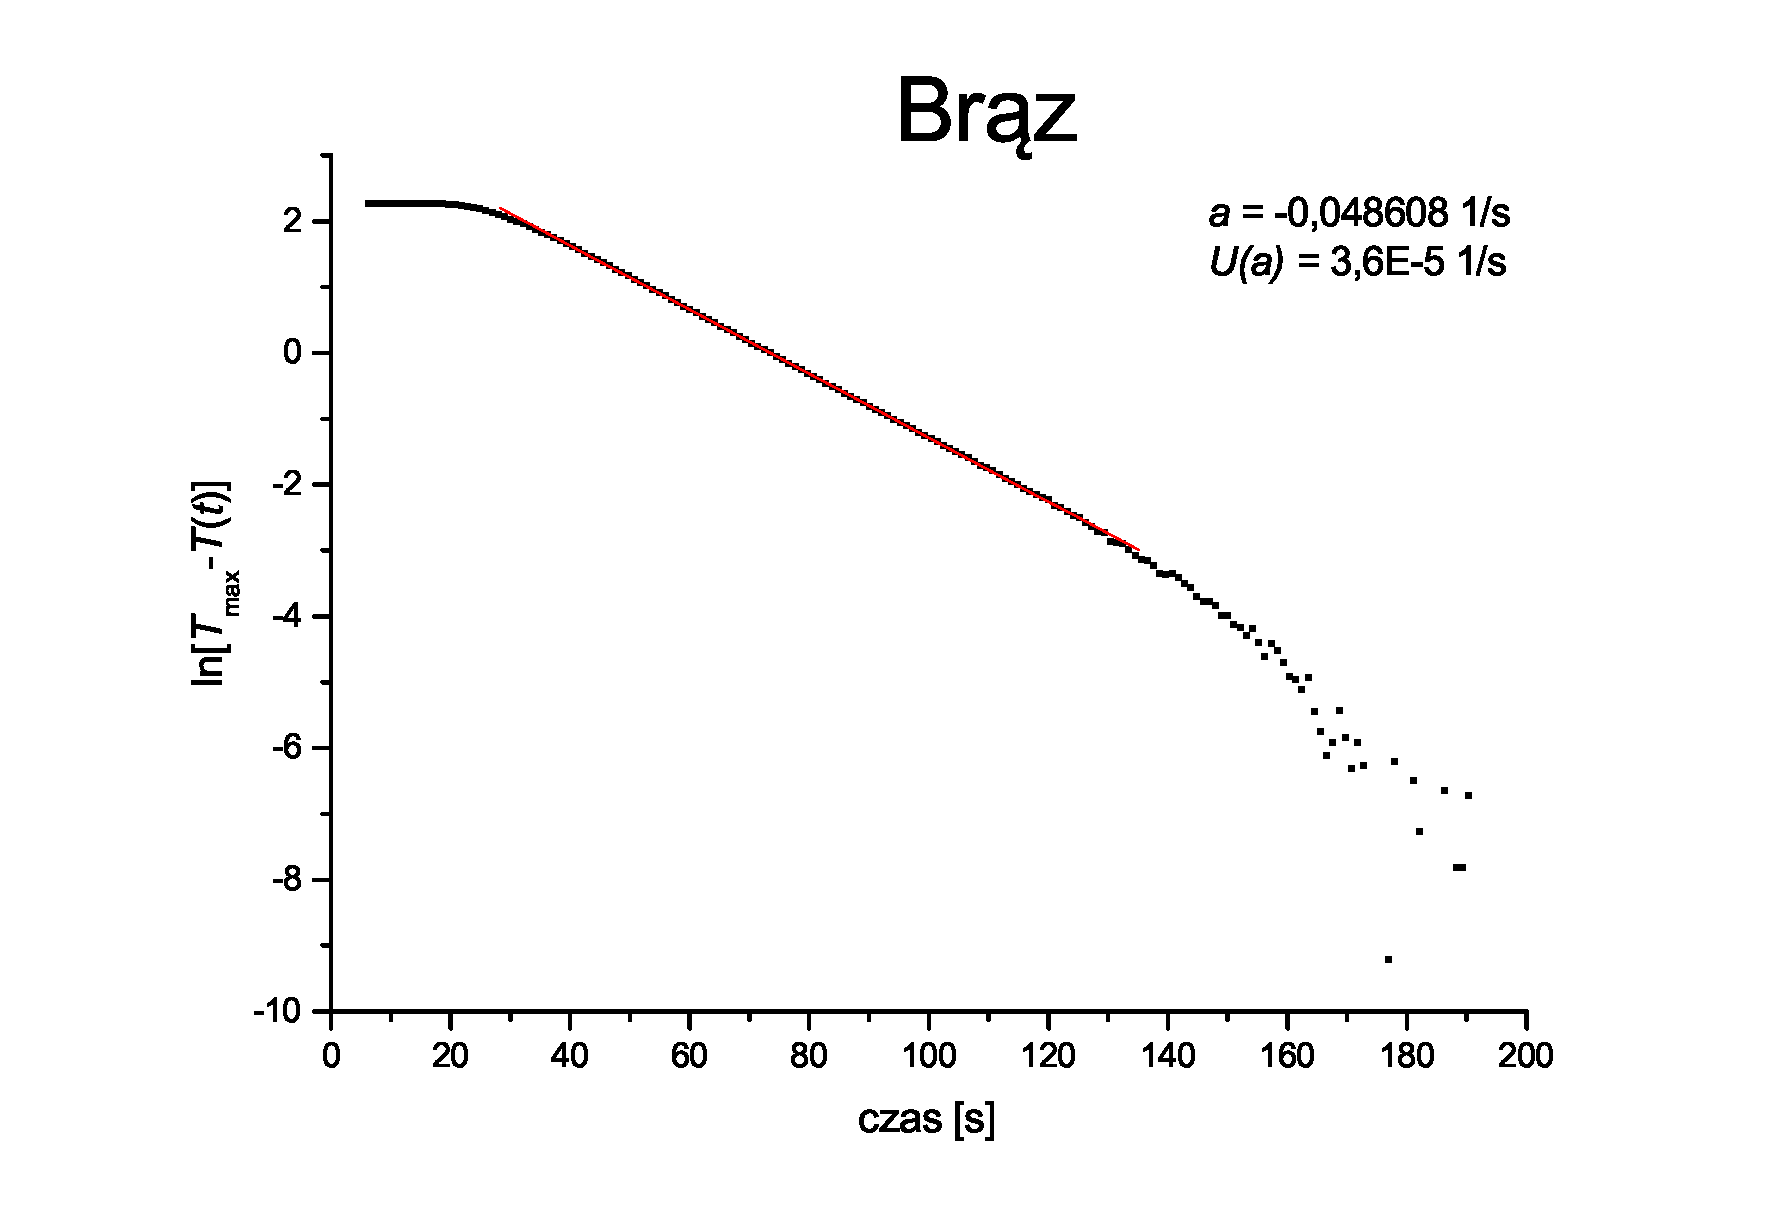
\includegraphics[height=0.4\textheight]{brazg.eps}
\caption{Wykres $\ln (T_{max} - T)$ w funkcji czasu dla próbki brązu}{\label{WYK_BRAZ}}
\end{center}
\end{figure}

\begin{figure}[h!]
\begin{center}
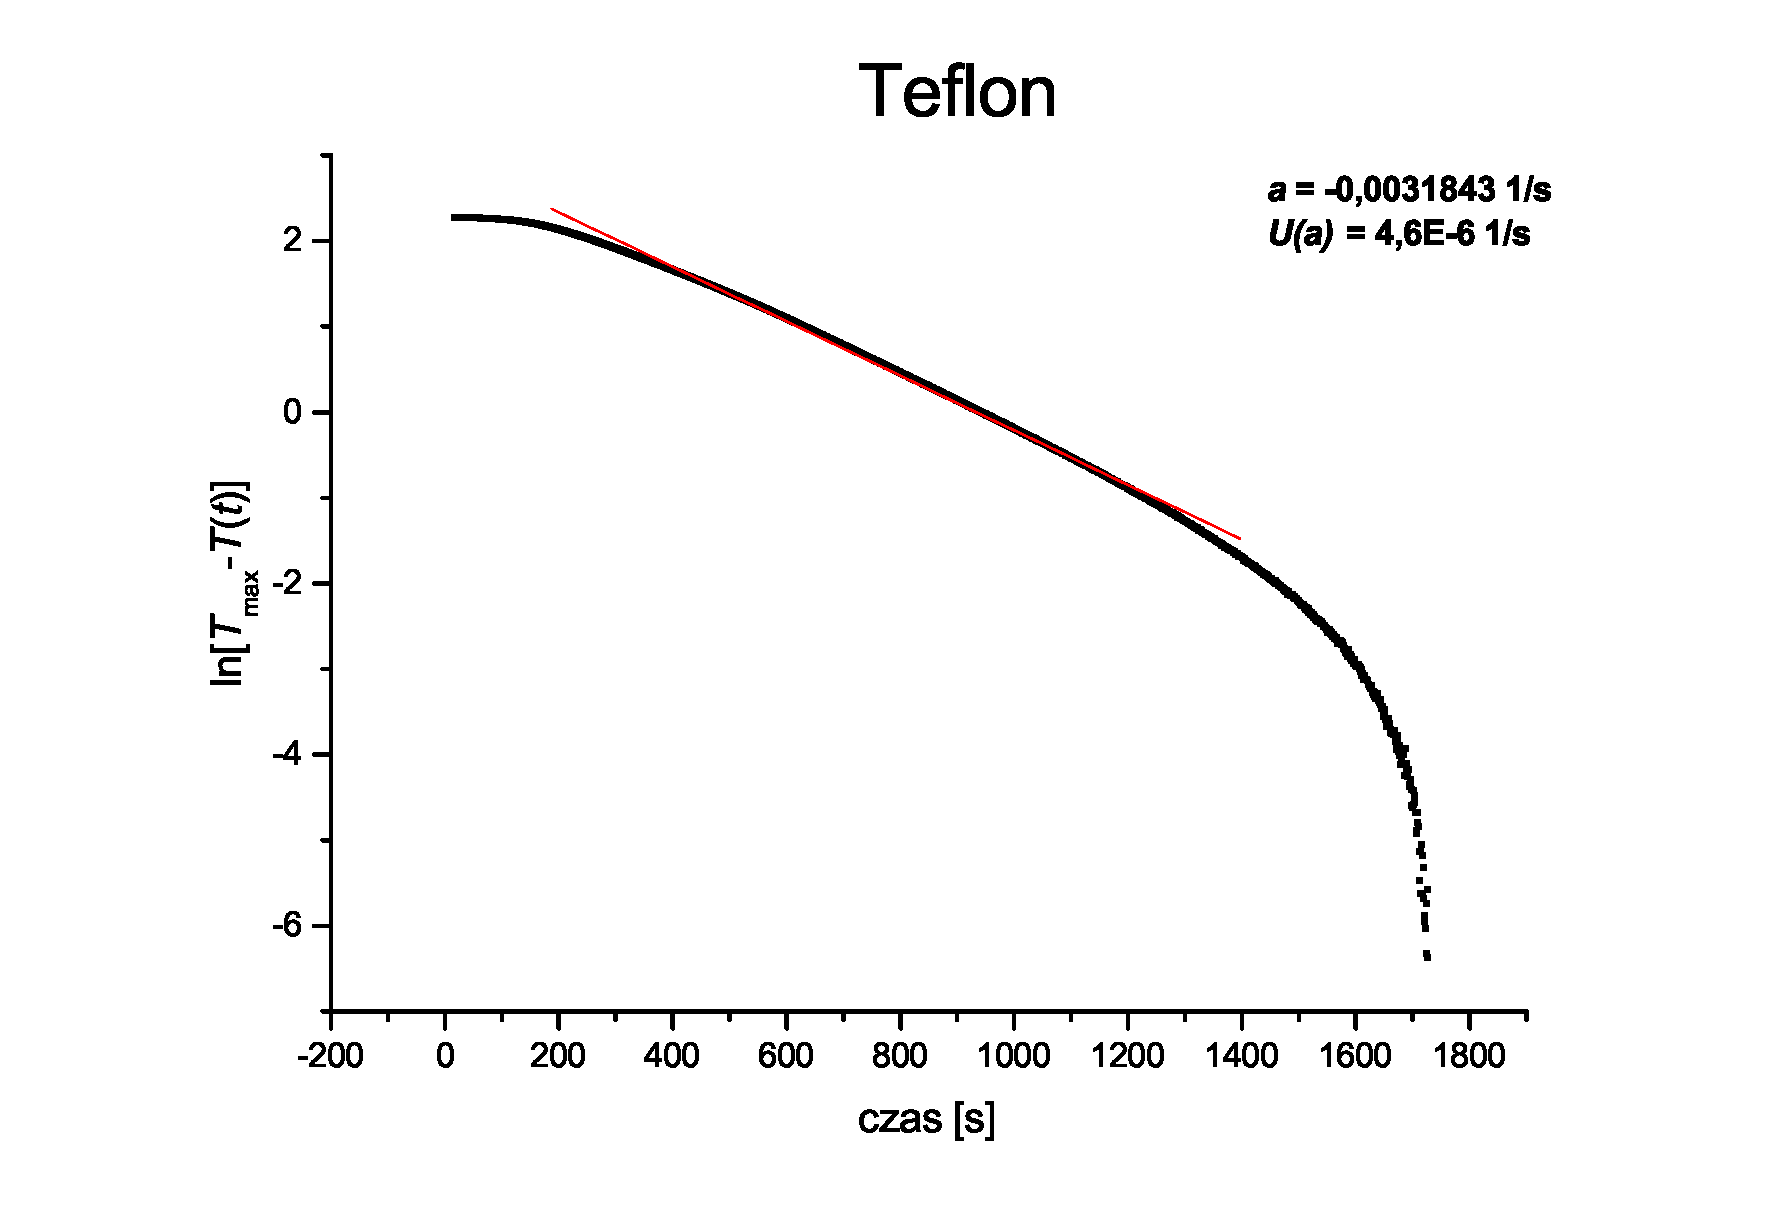
\includegraphics[height=0.4\textheight]{teflong.eps}
\caption{Wykres $\ln (T_{max} - T)$ w funkcji czasu dla próbki teflonu}{\label{WYK_TEFLON}}
\end{center}
\end{figure}

\begin{figure}[h!]
\begin{center}
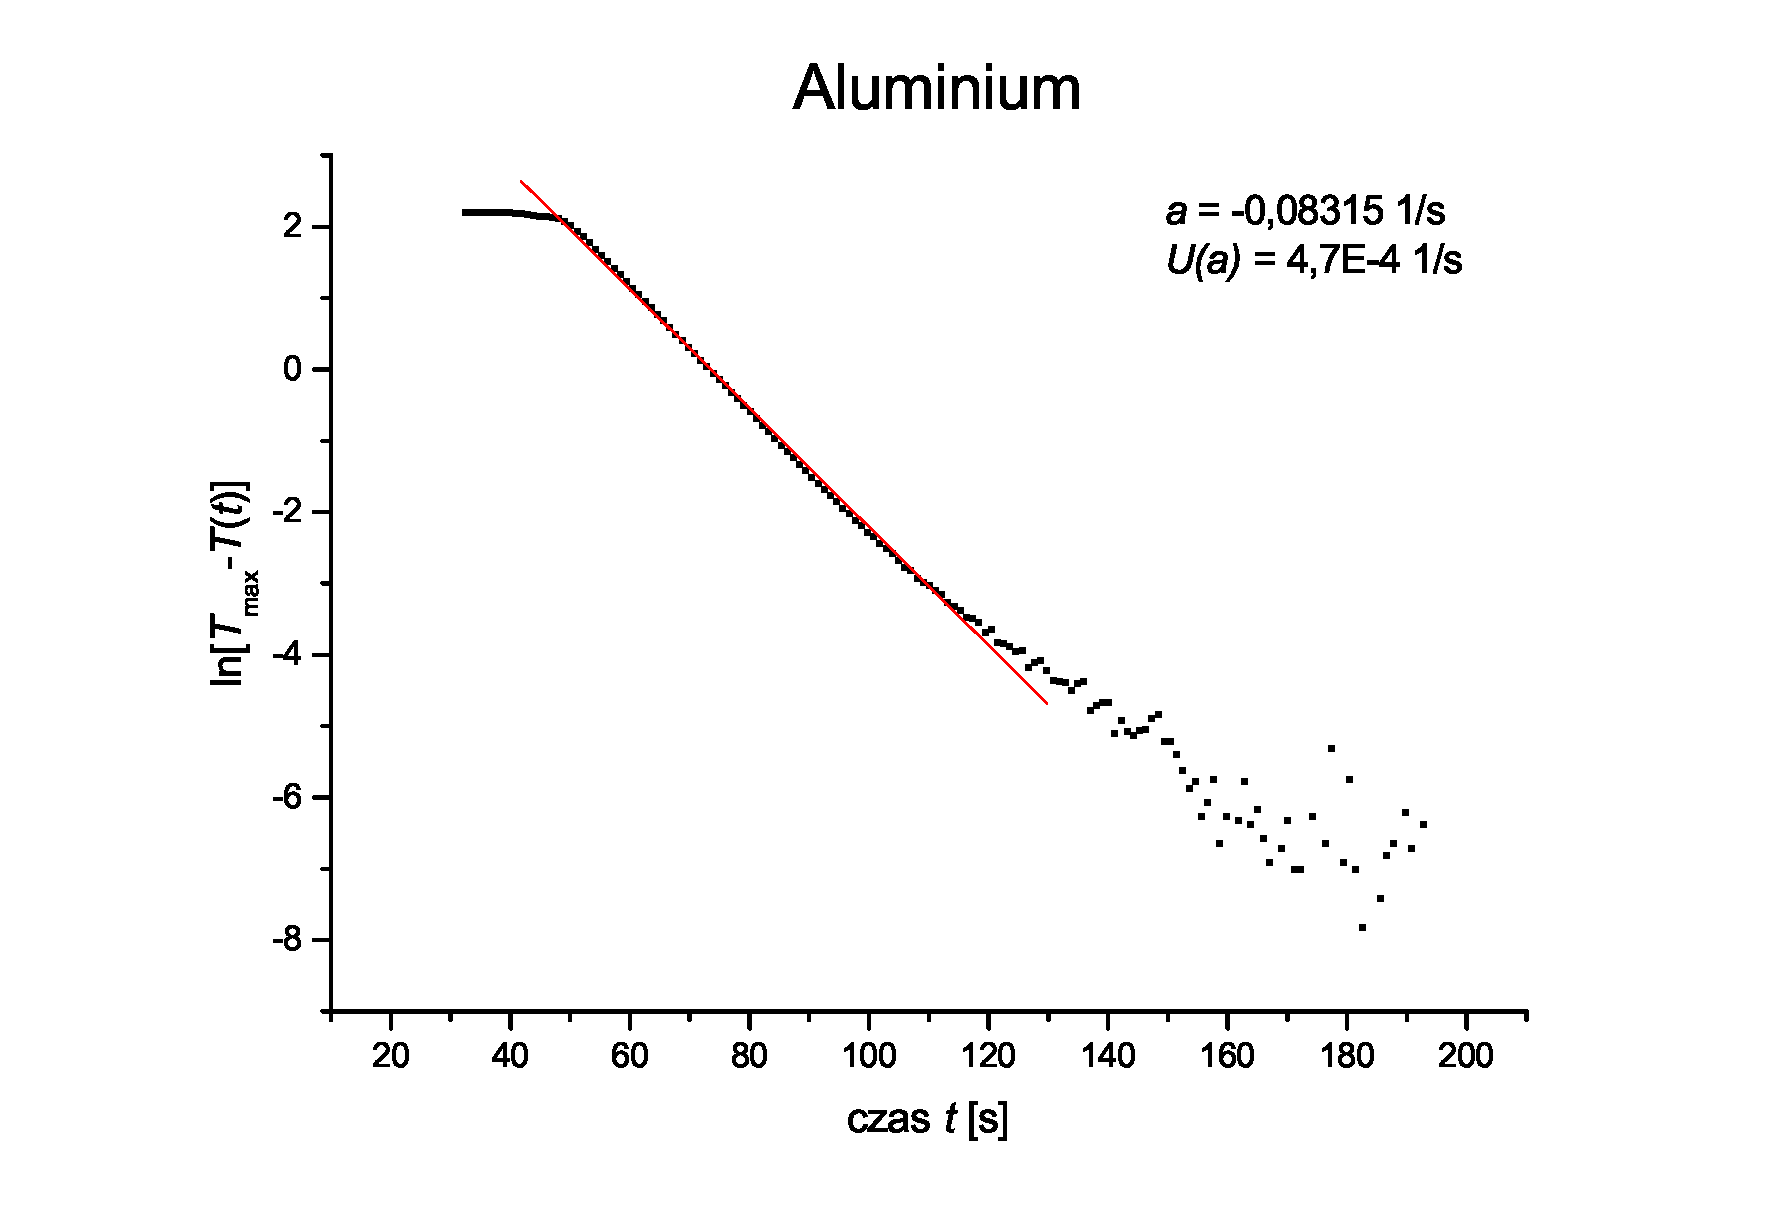
\includegraphics[height=0.4\textheight]{aluminiumg.eps}
\caption{Wykres $\ln (T_{max} - T)$ w funkcji czasu dla próbki aluminium}{\label{WYK_ALU}}
\end{center}
\end{figure}

\begin{figure}[h!]
\begin{center}
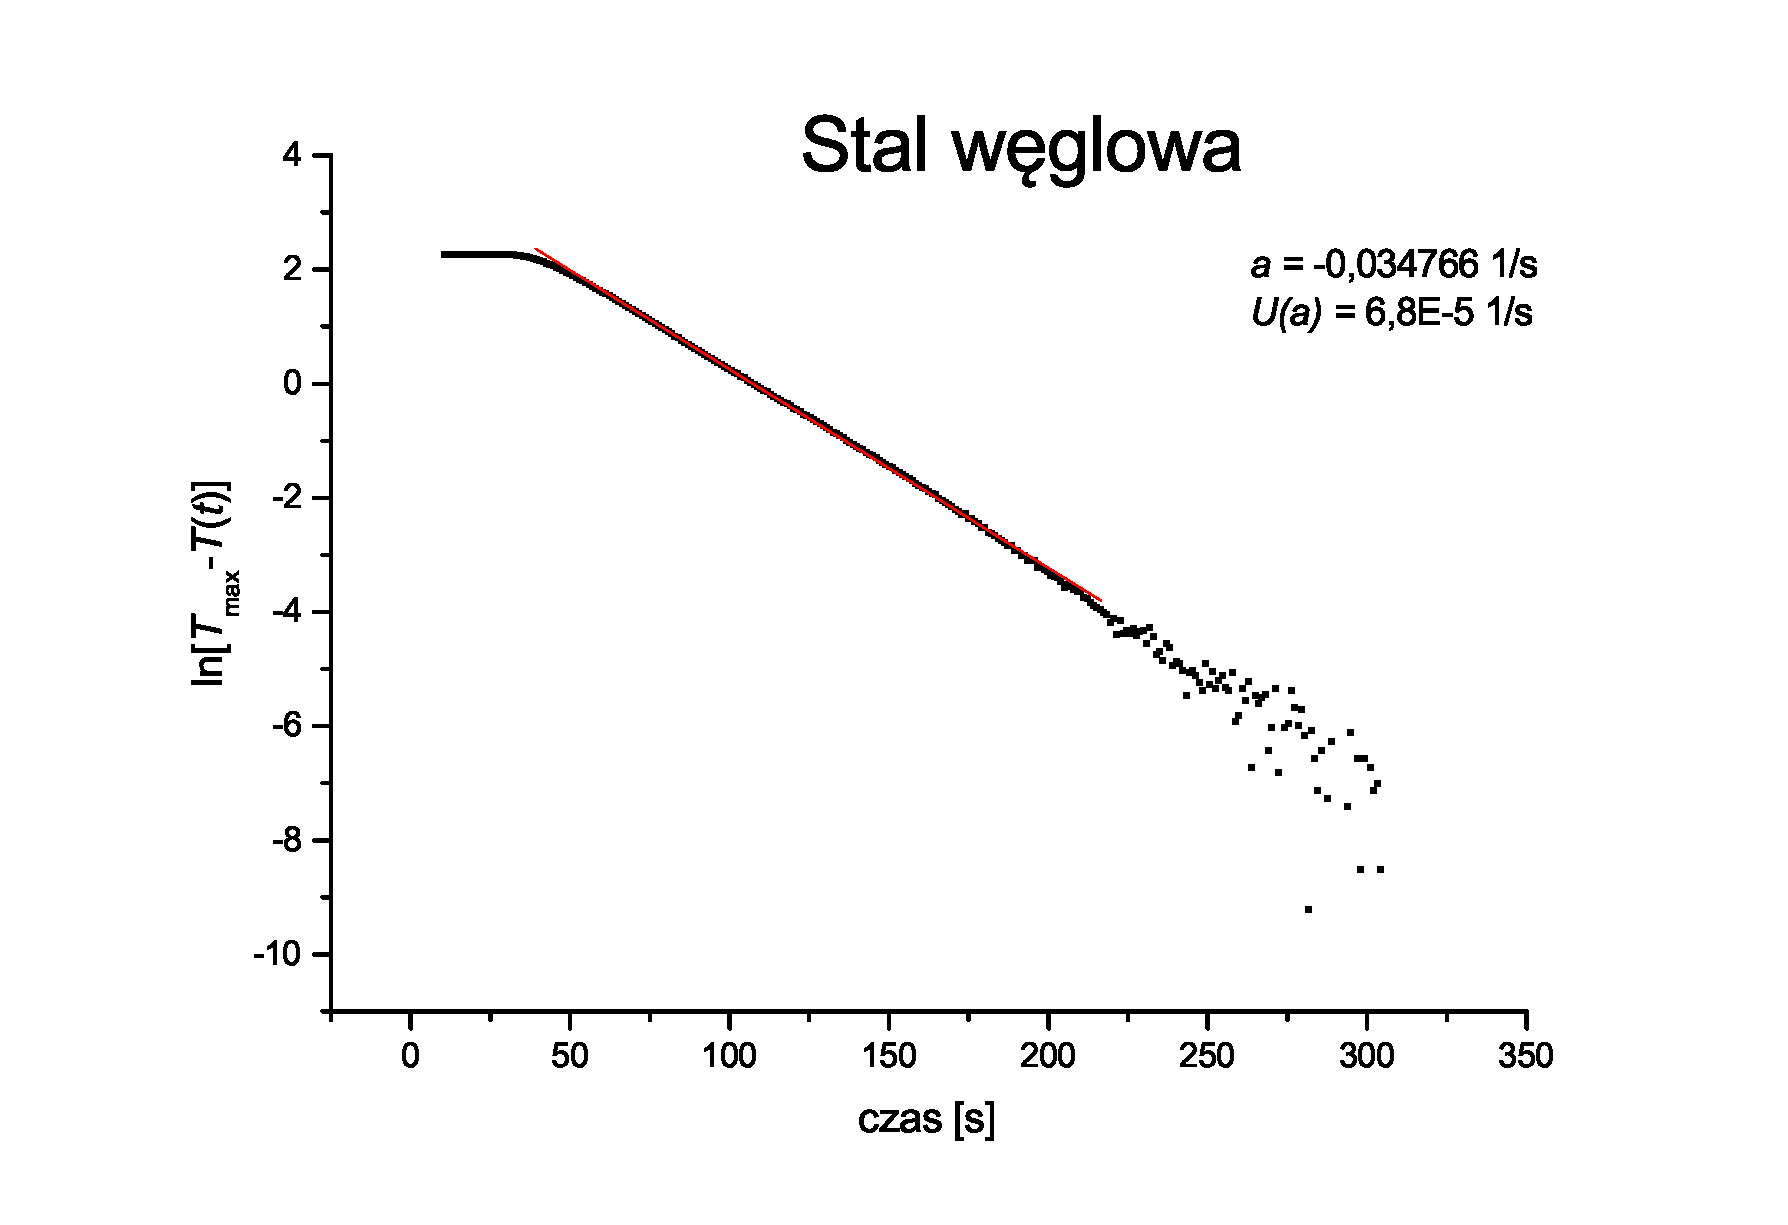
\includegraphics[height=0.4\textheight]{stal_weglowa.eps}
\caption{Wykres $\ln (T_{max} - T)$ w funkcji czasu dla próbki stali węglowej}{\label{WYK_STAL}}
\end{center}
\end{figure}

\begin{figure}[h!]
\begin{center}
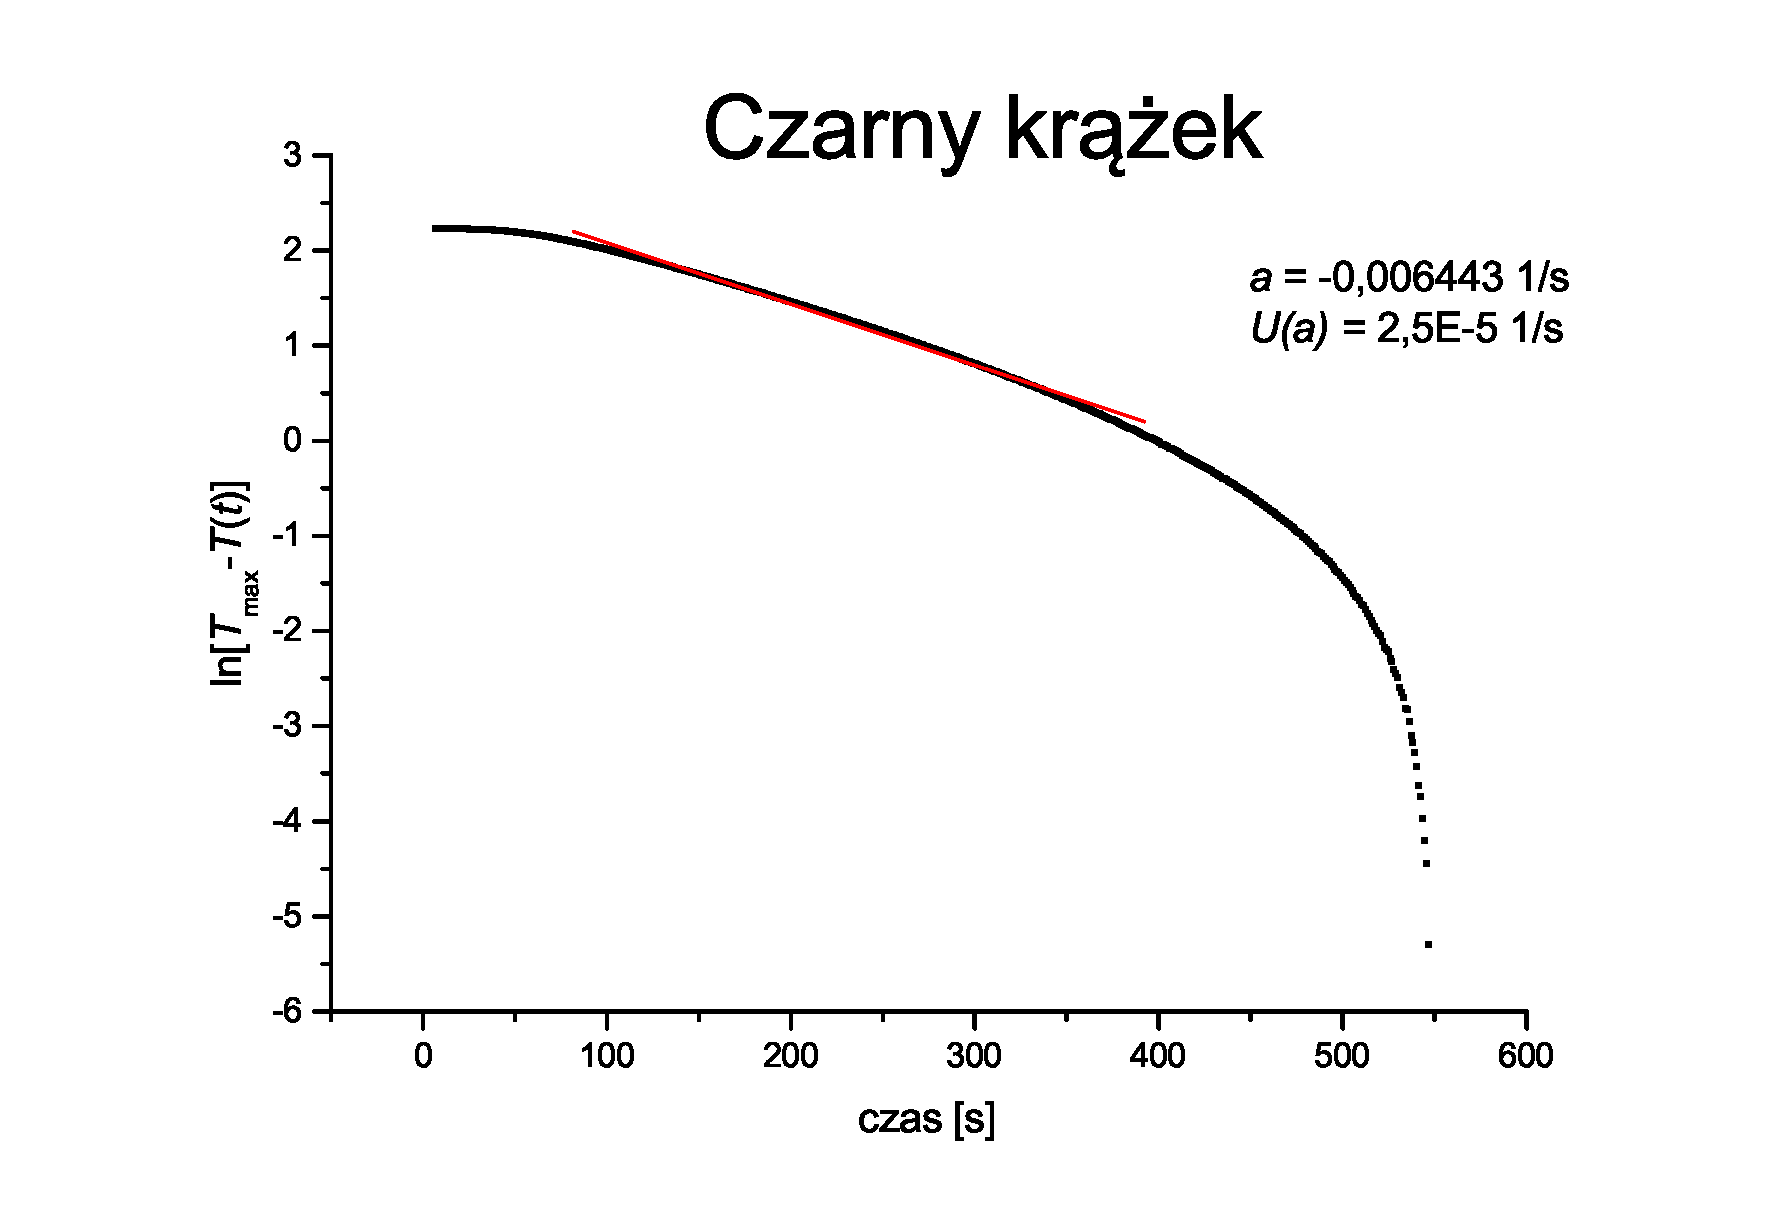
\includegraphics[height=0.4\textheight]{kronzekg.eps}
\caption{Wykres $\ln (T_{max} - T)$ w funkcji czasu dla czarnego krążka}{\label{WYK_CZK}}
\end{center}
\end{figure}

\begin{figure}[h!]
\begin{center}
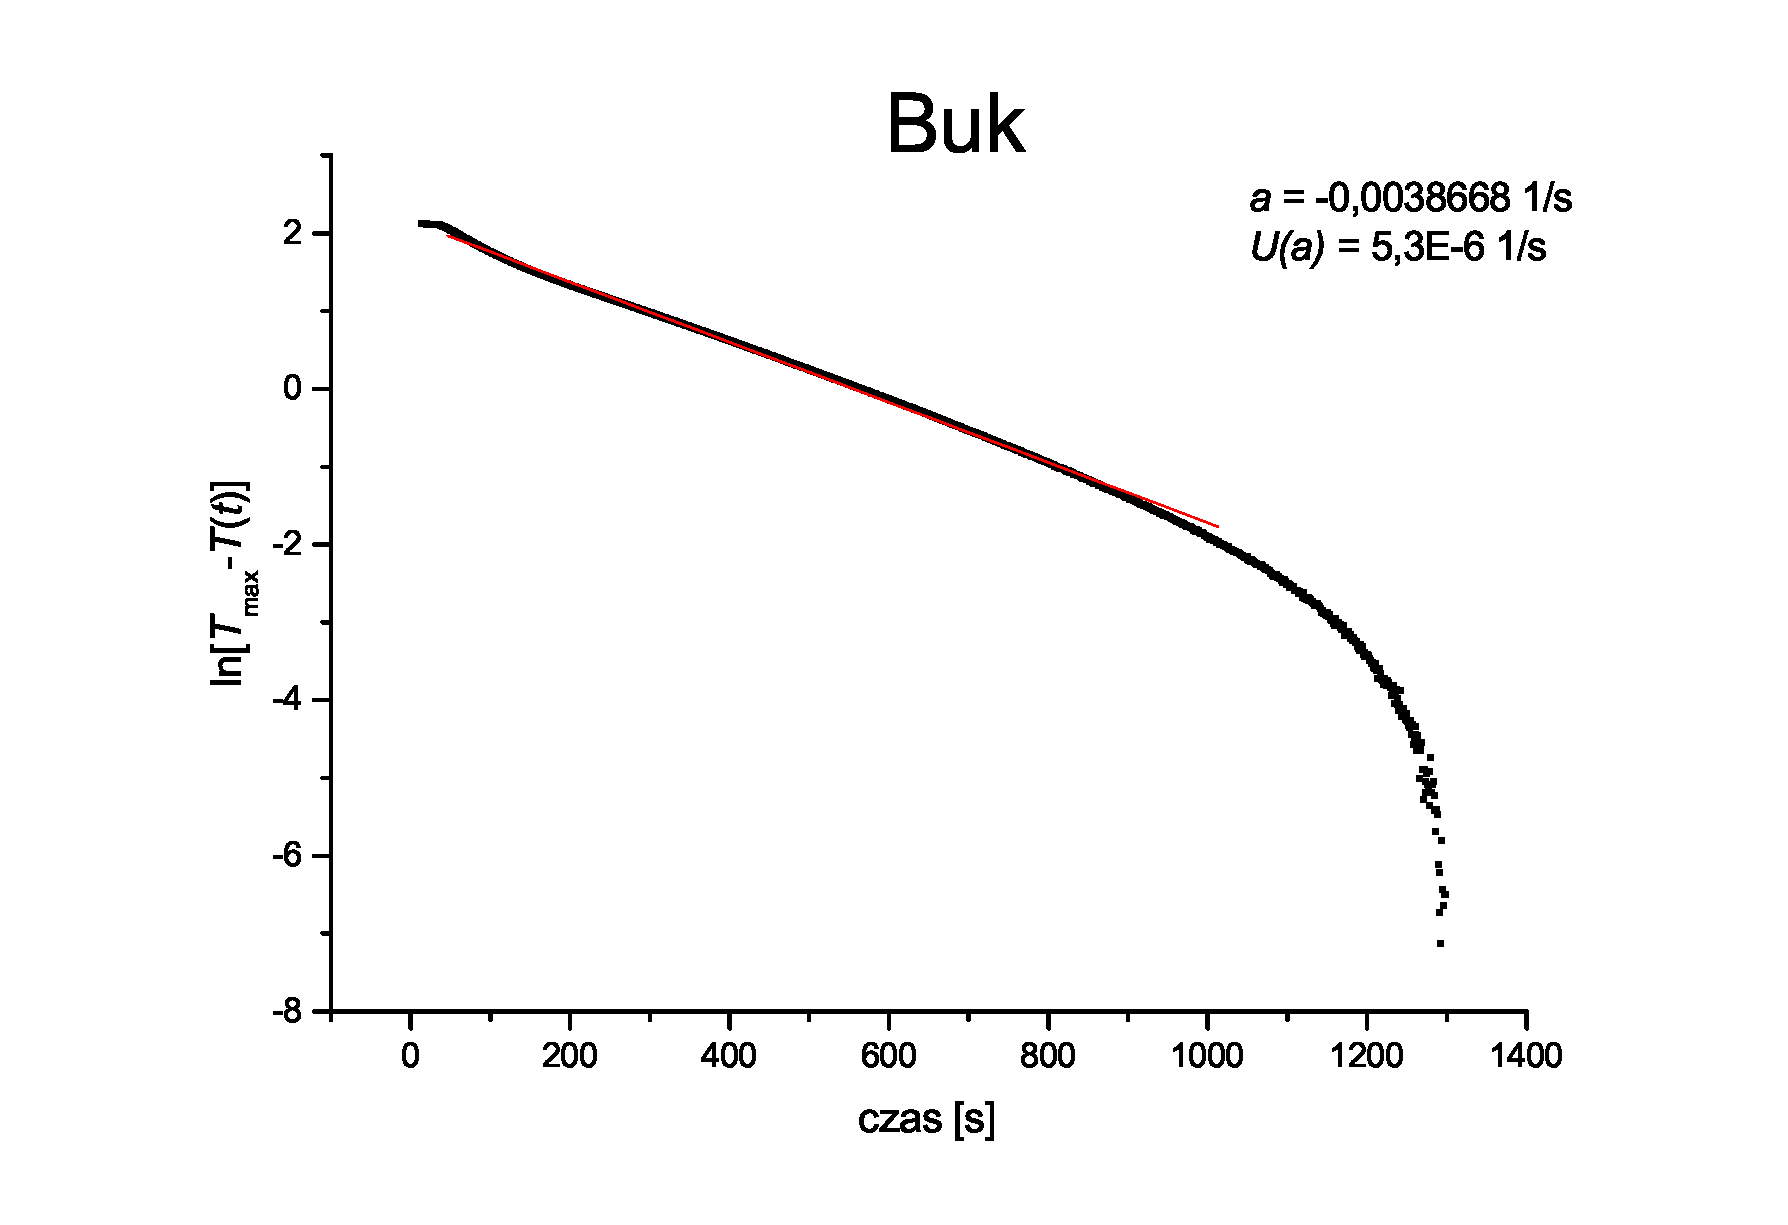
\includegraphics[height=0.4\textheight]{bukg.eps}
\caption{Wykres $\ln (T_{max} - T)$ w funkcji czasu dla kuli bukowej}{\label{WYK_BRAZ}}
\end{center}
\end{figure}
%%%%%%%%%%%%%%%%%%%%%%%%%%%%%%%%%%%%%%%%%%%%%%%%%%%%%%%%%%%%%%%%%%%%%%%%%%%%%%


\section*{Podsumowanie}
Wyniki zestawiono w tabeli \ref{TAB_K}. Dla teflonu otrzymane przewodnictwo
cieplne zgadza się z wartością tabelaryczną w granicach niepewności pomiarowych. 
Pozostałe wyniki zgadzają się z wartościami tabelarycznymi co do rzędu wielkości,
gdzie dla próbek stali węglowej, brązu i aluminium otrzymano wyniki zaniżone, a 
dla pozostałych zawyżone. Błędy te mogą wynikać z niedoskonałości geometrii badanych 
próbek lub drobnych zanieczyszczeń materiałów. W przypadku drewnianej kuli dodatkowym 
czynnikiem był lakier którym była pokryta jej powierzchnia.

\end{document}


